\section{Operation: high voltage, gain and sparks}\label{sec:operation}
\sectionstate{ready}{topic 6 (HV scans, \texttt{10\_hv\_scan\_*.py}); PLAN\_39 (\texttt{39\_spark\_deadtime.py}); spark waveforms (\texttt{40\_spark\_waveforms.py}); \texttt{det3\_spark\_analysis}}
\intent{Where the chambers run and why: efficiency plateau against spark rate, the chosen operating points,
and the evidence that the resistive layer does its job (sparks stay local and cost no dead time).}

\tbw{Mesh-voltage scans per chamber; plateaus and the chosen points (480/480/440\,V). Spark rate Poisson,
muon-induced (4--6$\times$), concentrated at the edges; no post-spark dead time.}
\askStephan{Expected gain curve and spark behaviour for this resistivity: does what we see match production tests?}

\begin{figure}[t]
  \centering
  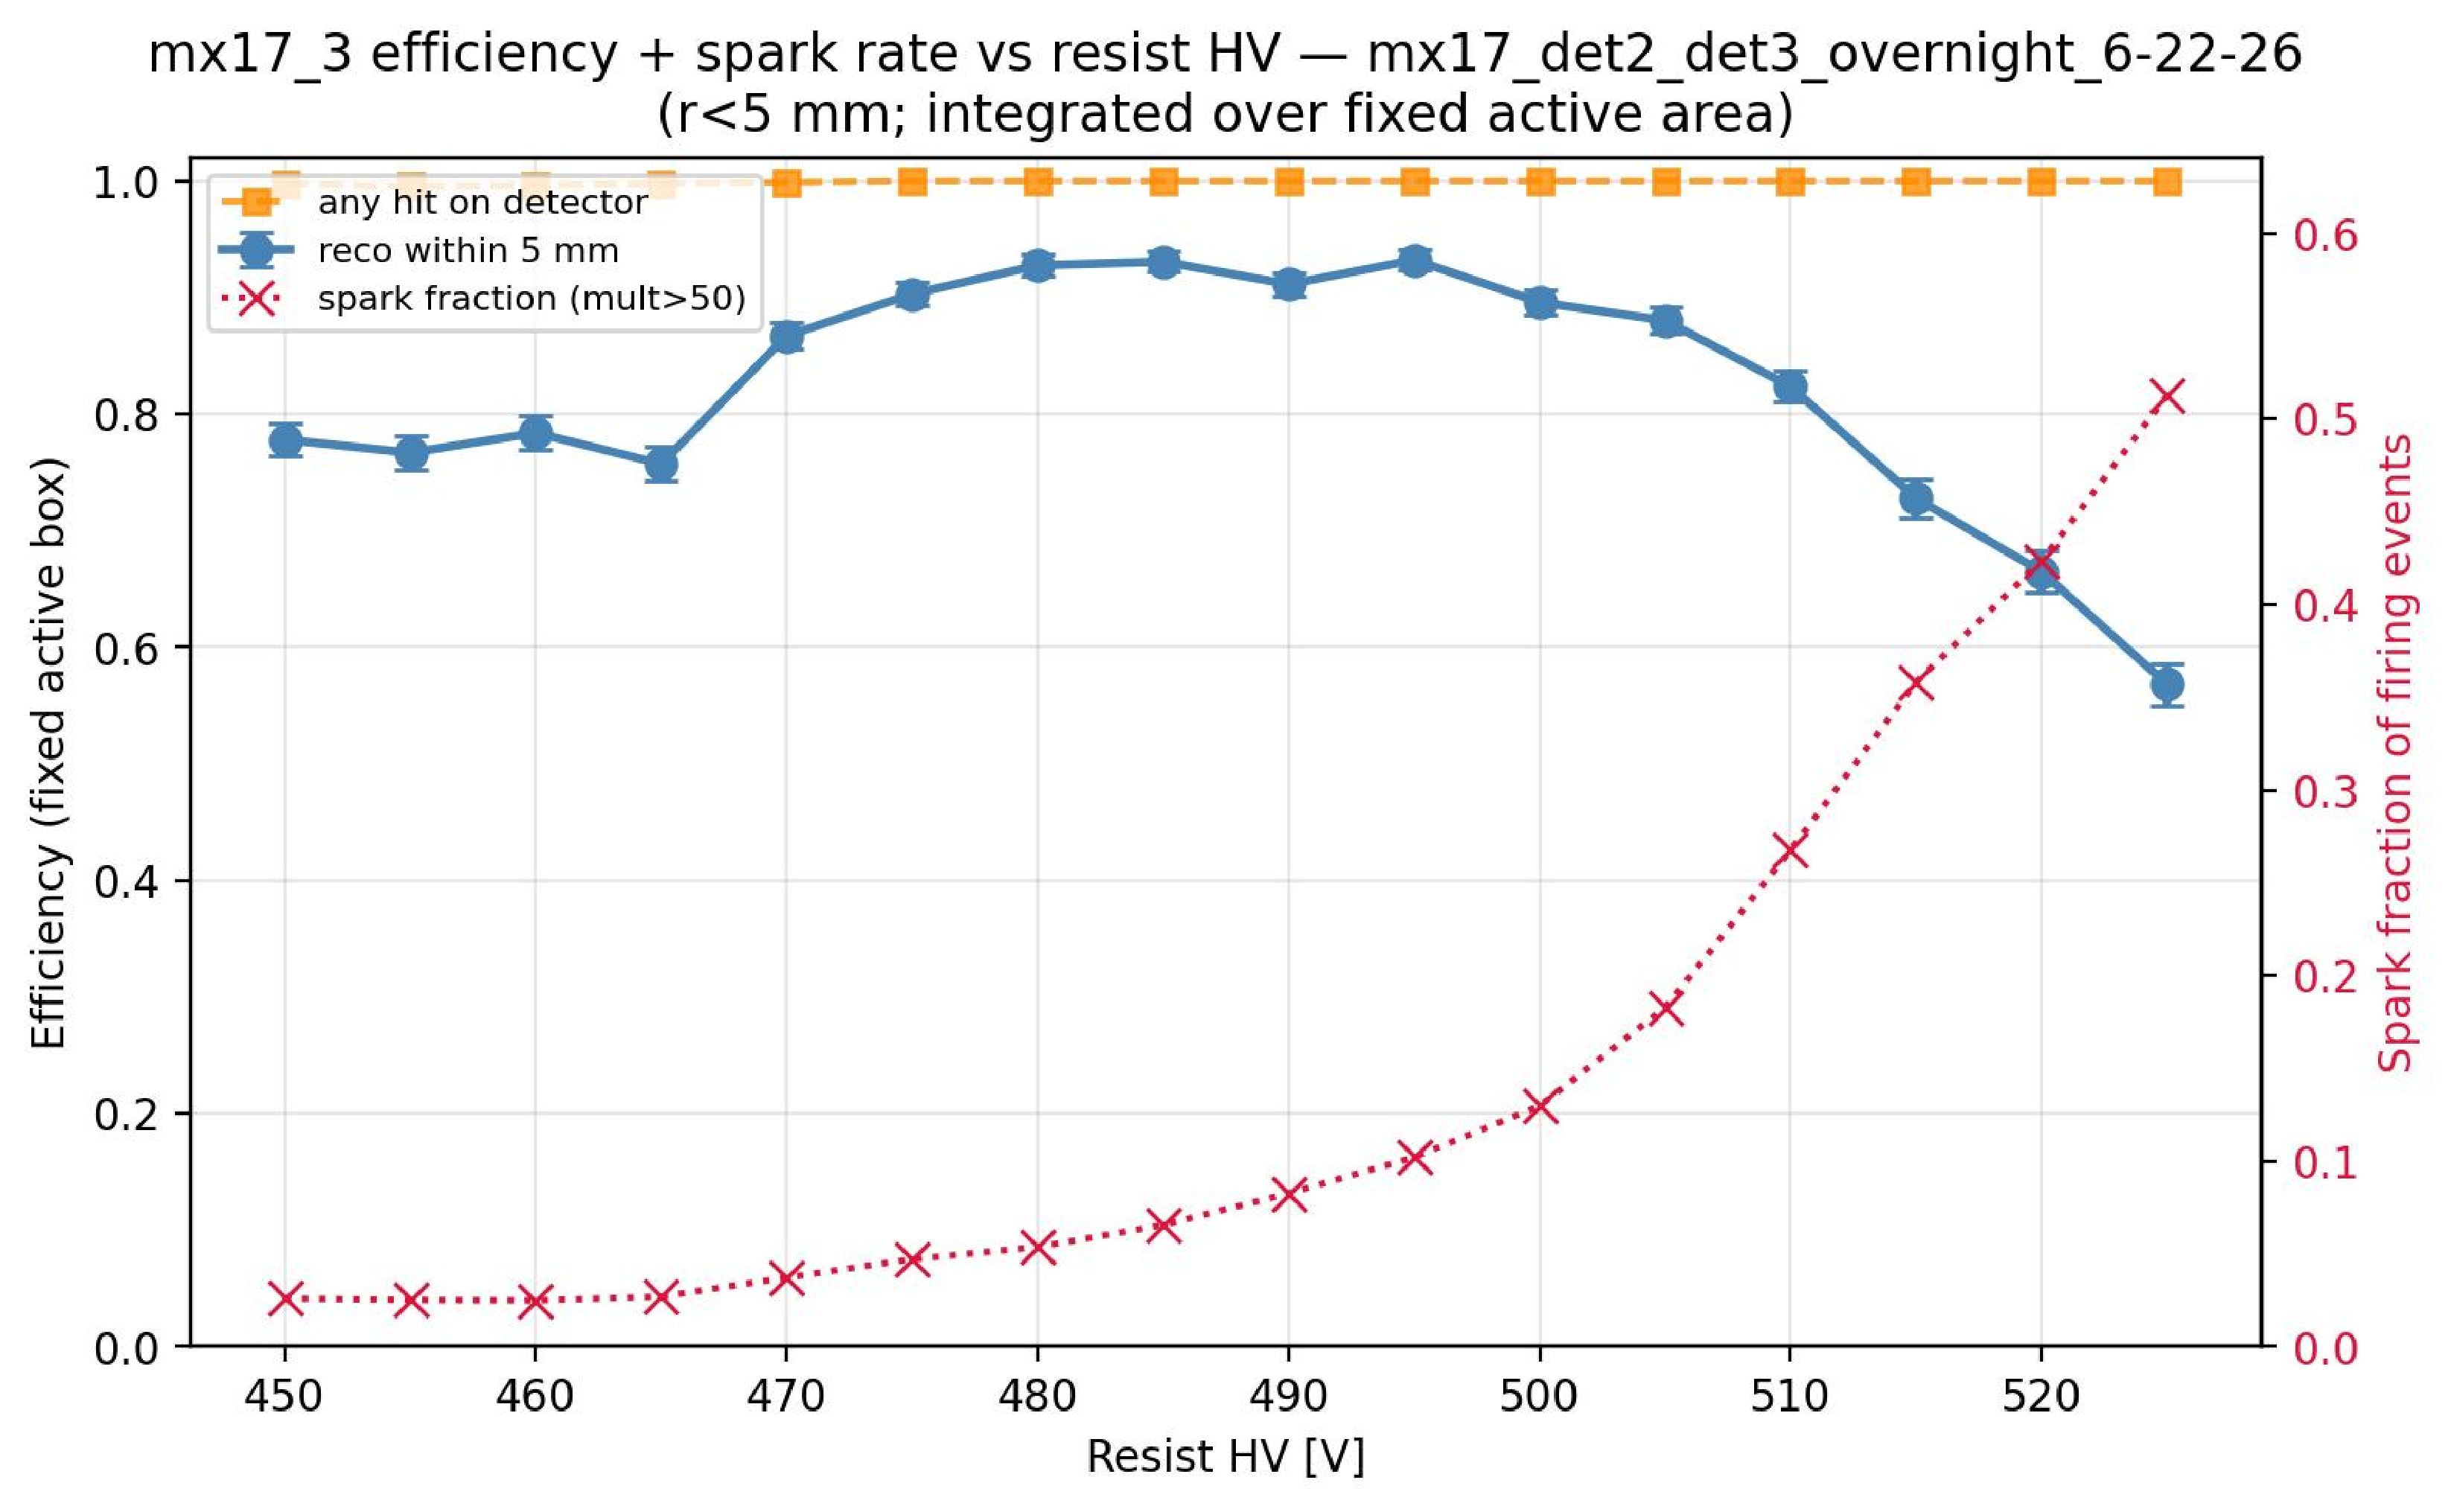
\includegraphics[width=0.75\linewidth]{hv_scan}
  \caption{\tbw{Mesh-voltage scan (det3): detection efficiency and spark rate.}}
  \label{fig:hv}
\end{figure}
\begin{figure}[t]
  \centering
  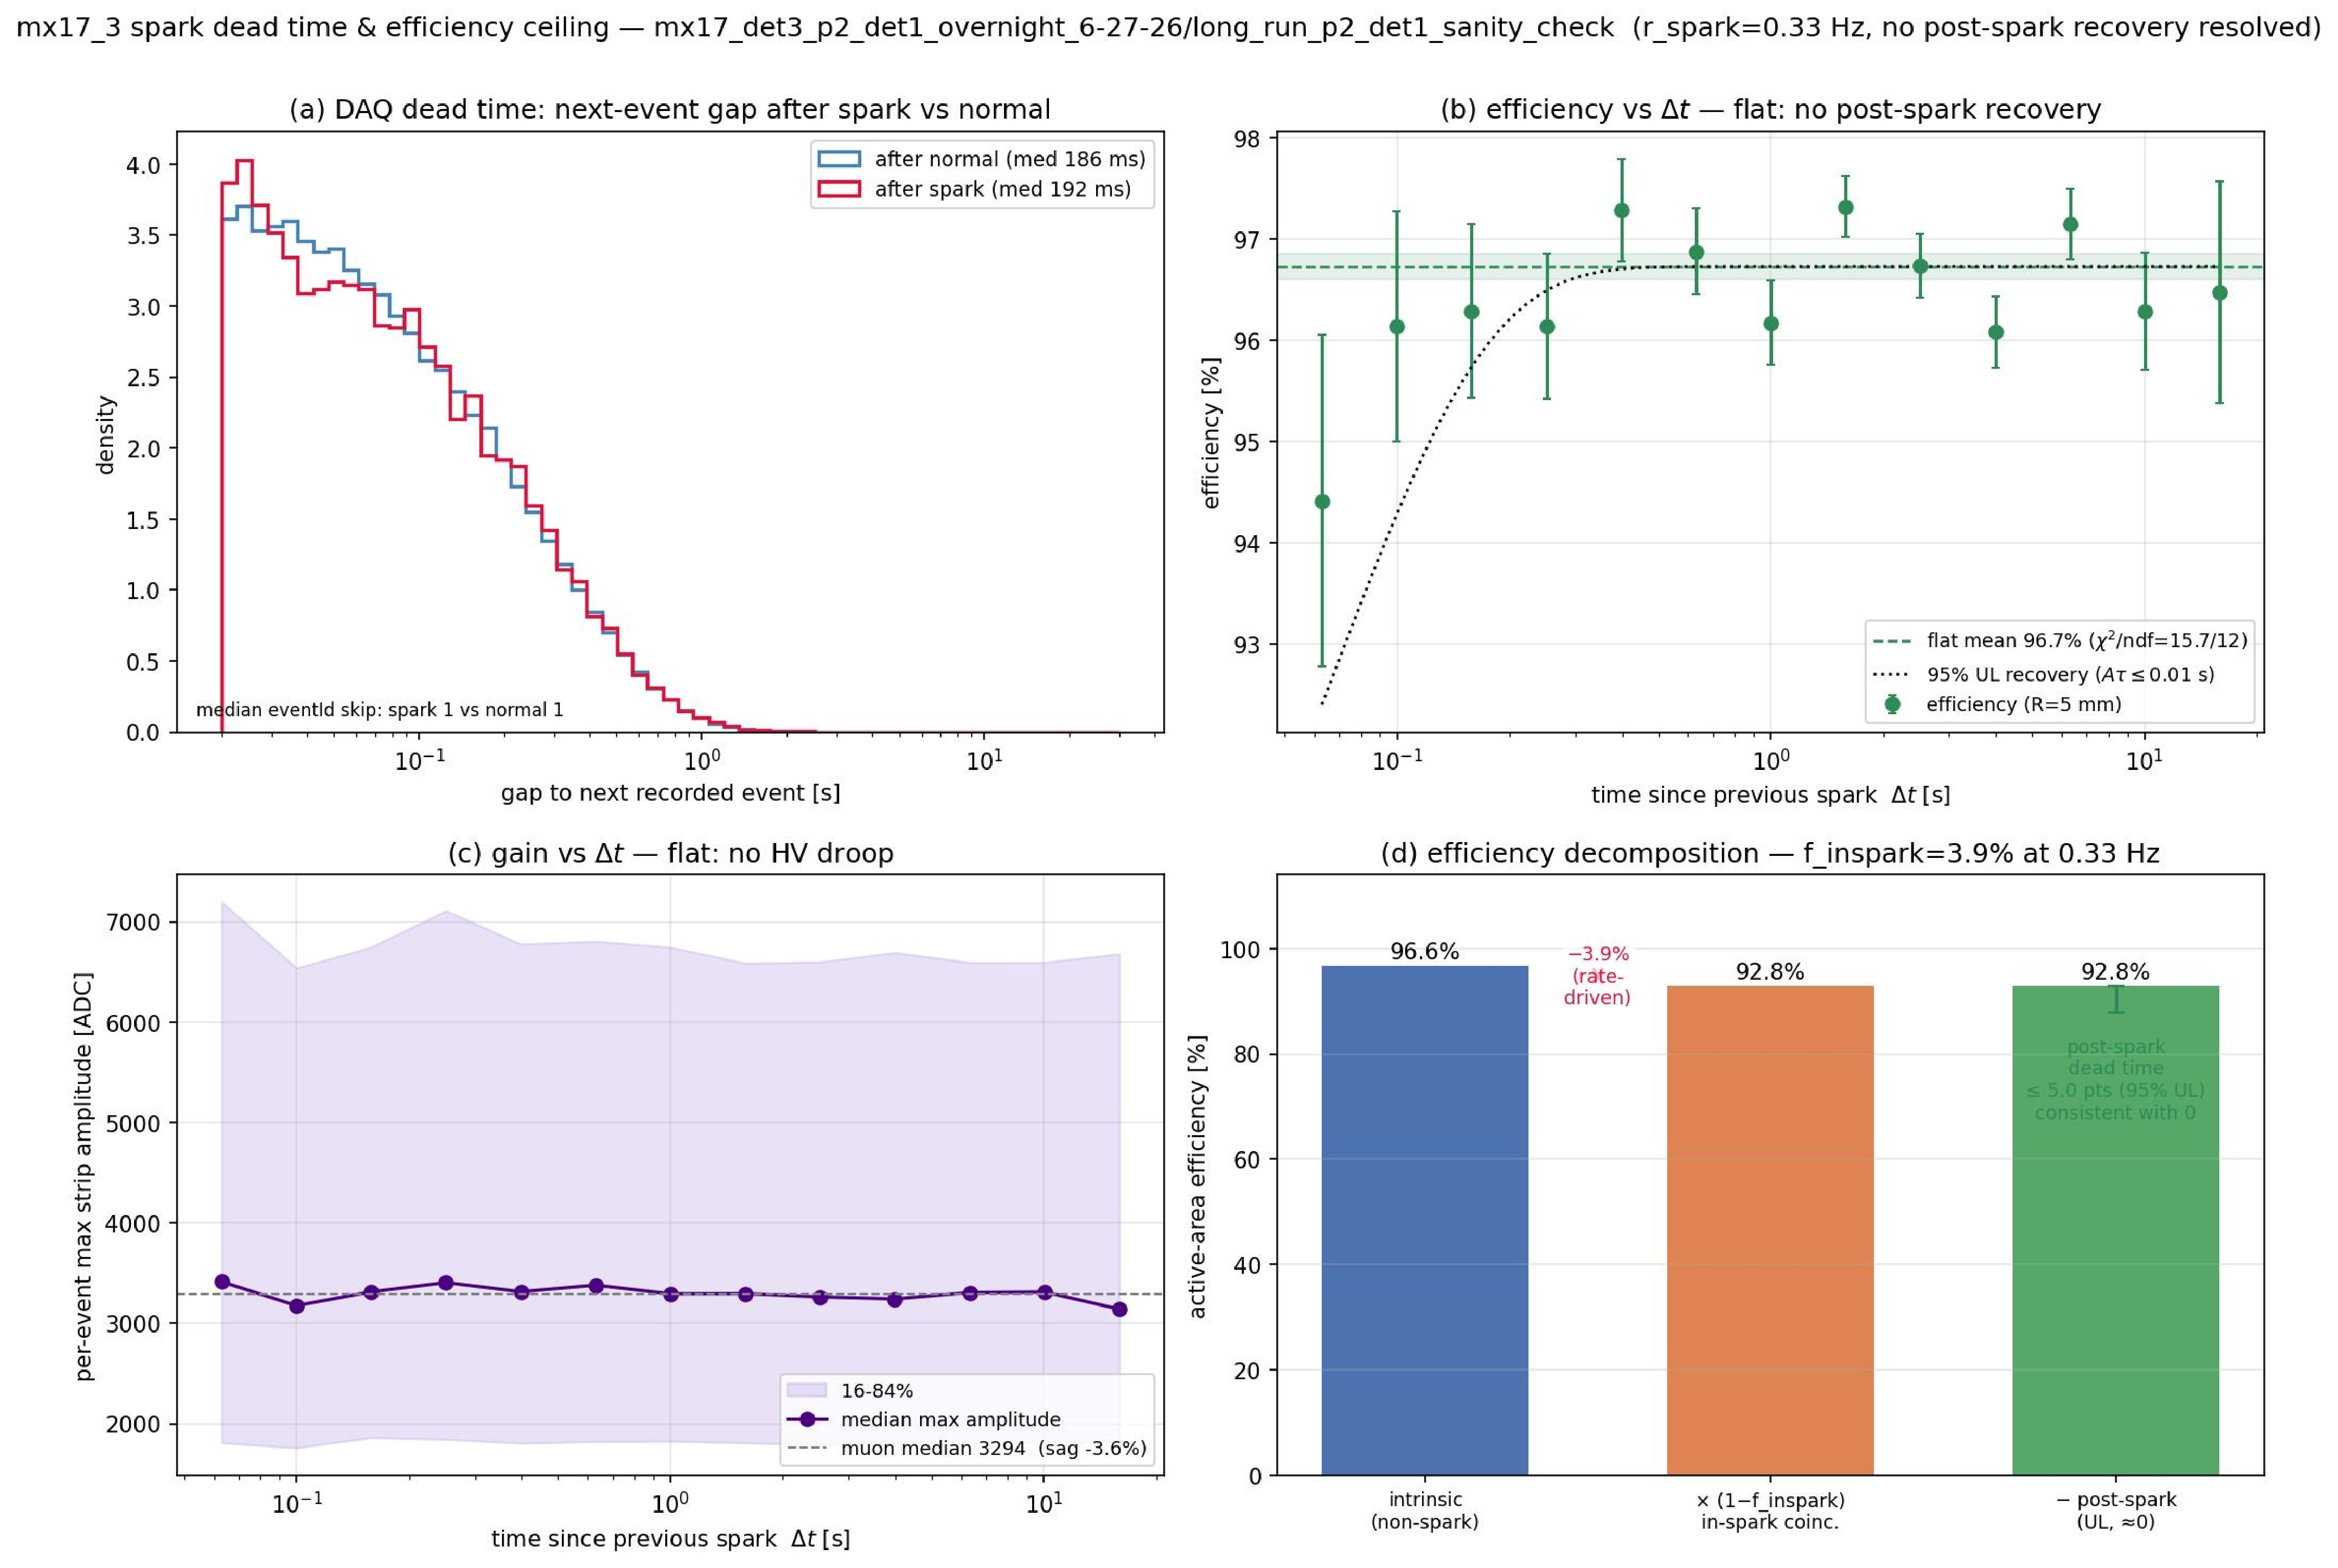
\includegraphics[width=0.75\linewidth]{spark_deadtime}
  \caption{\tbw{Efficiency in the time after a spark: no dead time.}}
  \label{fig:sparkdt}
\end{figure}
